\documentclass[10pt,a4paper]{article}
\usepackage[utf8]{inputenc}
\usepackage[spanish]{babel}
\usepackage{amsmath}
\usepackage{amsfonts}
\usepackage{amssymb}
\usepackage{graphicx}
\usepackage{float}
\usepackage{listings}
\usepackage{color}

\definecolor{codegreen}{rgb}{0,0.6,0}
\definecolor{codegray}{rgb}{0.5,0.5,0.5}
\definecolor{codepurple}{rgb}{0.58,0,0.82}
\definecolor{backcolour}{rgb}{0.95,0.95,0.92}
\author{Liliana Carolina Saus Olvera }
\title{Tarea 1: Representación de redes a través de la teoría de grafos}
\lstdefinestyle{mystyle}{
    backgroundcolor=\color{backcolour},   
    commentstyle=\color{codegreen},
    keywordstyle=\color{magenta},
    numberstyle=\tiny\color{codegray},
    stringstyle=\color{codepurple},
    basicstyle=\footnotesize,
    breakatwhitespace=false,         
    breaklines=true,                 
    captionpos=b,                    
    keepspaces=true,                 
    numbers=left,                    
    numbersep=5pt,                  
    showspaces=false,                
    showstringspaces=false,
    showtabs=false,                  
    tabsize=2
}

\lstset{style = mystyle}

\begin{document}
\maketitle
Objetivo: Se identifica aplicaciones prácticas para los siguientes tipos de grafos y se representa un ejemplo inspirado en datos reales para cada caso, con por lo menos cinco vértices y no más de doce vértices por caso

%%1
\section{Grafo simple no dirigido acíclico}
\subsection{Ejemplo} Las lineas del metro en Nuevo León son una representación de este tipo grafo, en donde las estaciones representan cada uno de los nodos y la distancia entre estas estaciones representan las aristas, una característica de las lineas del metro es que son acíclicas y se mueven en dos direcciones.

\subsection{Código}\lstinputlisting[language=Python]{2.py}
\begin{figure}[H]
\centering
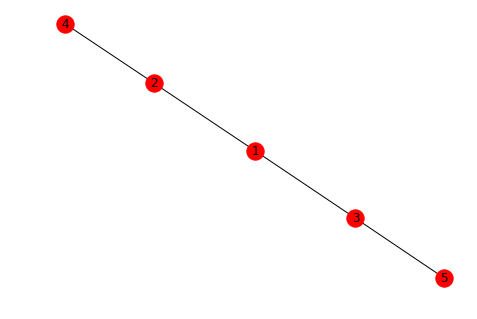
\includegraphics[scale=.5]{grafosimplenodirigidoaciclico}
\caption{Gráfo simple no dirigido acíclico}
\end{figure}

%%2
\section{Gráfo Simple no dirigido cíclico}
\subsection{Ejemplo} En múltiples lugares de servicio se tienen rutas, las cuales empiezan y terminan en un mismo lugar,esto puede representar un grafo simple no dirigido acíclico, en donde los nodos son los lugares que se debe visitar y las aristas, la distancia de dirigirse a cada lugar.
\subsection{Código}\lstinputlisting[language=Python]{1.py}
\begin{figure}[H]
\centering
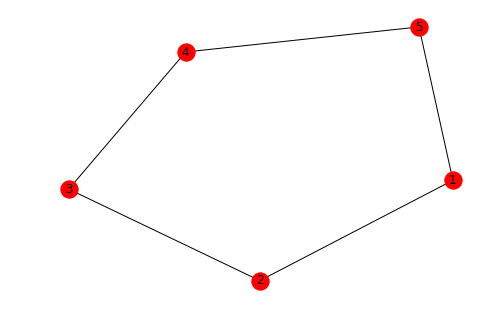
\includegraphics[scale=.5]{grafosimplenodirigidociclico}
\caption{Gráfo simple no dirigido cíclico}
\end{figure}

%%3
\section{Simple no dirigido reflexivo}
\subsection{Código}\lstinputlisting[language=Python]{3.py}
\begin{figure}[H]
\centering
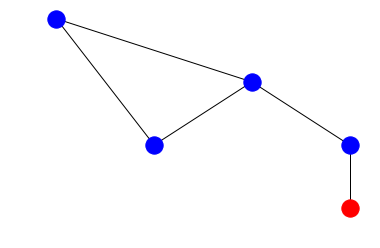
\includegraphics[scale=.5]{grafosimplenodirigidoreflexivo}
\caption{Gráfo simple no dirigido reflexivo}
\end{figure}

%%4
\section{Grafo simple  dirigido acíclico}
\subsection{Ejemplo}Las lineas del metro en Nuevo León representan este tipo de grafo, donde se toma en cuenta solo una dirección del metro, por ejemplo la ruta de ir de la estación Anahuac a  Anaya, donde las aristas es la dirección entre cada estación y los nodos son las estaciones. 
\subsection{Código}\lstinputlisting[language=Python]{4.py}
\begin{figure}[H]
\centering
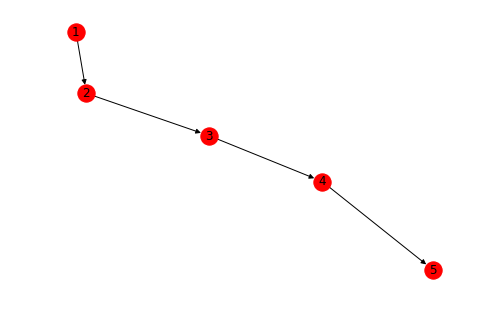
\includegraphics[scale=.5]{grafosimpledirigidoaciclico}
\caption{Gráfo simple dirigido acíclico}
\end{figure}

%%5
\section{Grafo simple  dirigido cíclico}
\subsection{Ejemplo} La ruta del camión 213 es un ejemplo, ya que su recurrido es un ciclo y las paradas consecutivas representan los nodos y la distancia entre estas paradas las aristas. 
\subsection{Código}\lstinputlisting[language=Python]{5.py}
\begin{figure}[H]
\centering
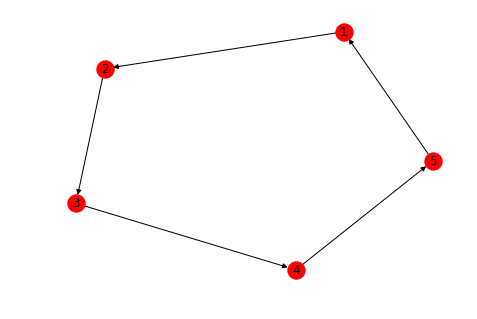
\includegraphics[scale=.5]{grafosimpledirigidociclico}
\caption{Gráfo simple  dirigido cíclico}
\end{figure}

%%6
\section{Grafo simple dirigido reflexivo}
\subsection{Ejemplo} La órbita de la tierra representa este tipo de grafo, donde el movimiento que hace en girar en si misma, da lugar a reflexividad. 
\subsection{Código}\lstinputlisting[language=Python]{6.py}
\begin{figure}[H]
\centering
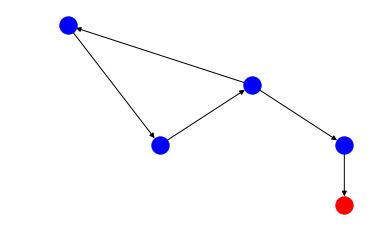
\includegraphics[scale=.5]{grafosimpledirigidoreflexivo}
\caption{Gráfo simple  reflexivo}
\end{figure}

%%7
\section{Multigrafo no dirigido acíclico}
\subsection{Ejemplo} La linea 1 y la linea 2 del metro, su recorrido representa un ,multigrafo no dirigido aciclico.
\subsection{Código}\lstinputlisting[language=Python]{7.py}
\begin{figure}[H]
\centering
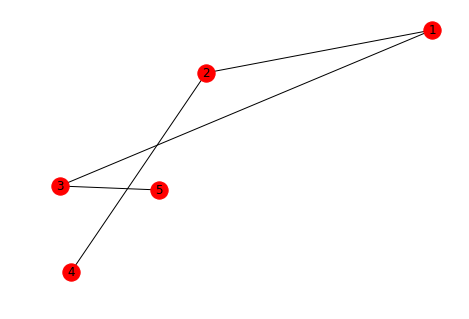
\includegraphics[scale=.5]{multigrafonodirigidoaciclico}
\caption{Multigrafo no dirigido acíclico}
\end{figure}

%%8
\section{Multigrafo no dirigido cíclico}
\subsection{Ejemplo} En ocasiones existen distintas alternativas para llegar a un mismo lugar, como lo es la vialidad en Nuevo León, el cual podemos consider como un multigrafo no dirigido aciclico. 
\subsection{Código}\lstinputlisting[language=Python]{8.py}
\begin{figure}[h]
\centering
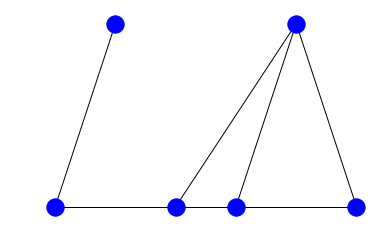
\includegraphics[scale=.5]{multigrafonodirigidociclico}
\caption{Multigrafo no dirigido cíclico}
\end{figure}

%%9
\section{Multigrafo no dirigido reflexivo}
\subsection{Código}\lstinputlisting[language=Python]{9.py}
\begin{figure}[H]
\centering
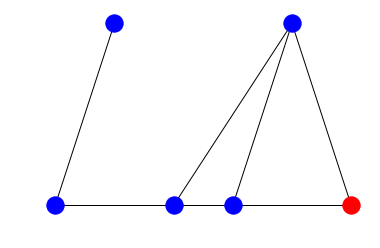
\includegraphics[scale=.5]{multigrafonodirigidoreflexivo}
\caption{Multigrafo no dirigido reflexivo}
\end{figure}

%%10
\section{Multigrafo dirigido acíclico}
\subsection{Ejemplo} La red de tuberías de pluvial, donde los nodos son puntos de presión para impulsar el agua hacia los destinos y las son las tuberías. 
\subsection{Código}\lstinputlisting[language=Python]{10.py}
\begin{figure}[H]
\centering
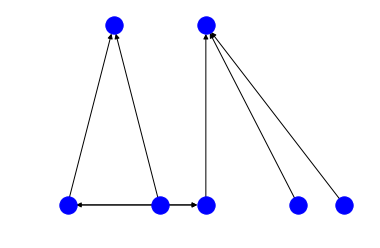
\includegraphics[scale=.5]{multigrafodirigidoaciclico}
\caption{Multigrafo dirigido acíclico}
\end{figure}

%%11
\section{Multigrafo dirigido cíclico}
\subsection{Código}\lstinputlisting[language=Python]{11.py}
\begin{figure}[H]
\centering
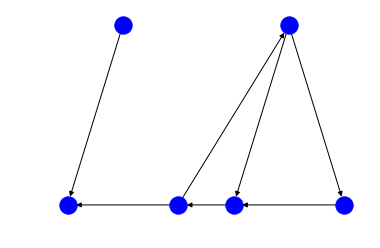
\includegraphics[scale=.5]{multigrafodirigidociclico}
\caption{Multigrafo dirigido cíclico}
\end{figure}

%%12
\section{Multigrafo dirigido reflexivo}
\subsection{Código}\lstinputlisting[language=Python]{12.py}
\begin{figure}[H]
\centering
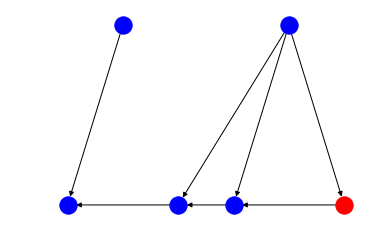
\includegraphics[scale=.5]{multigrafodirigidoreflexivo}
\caption{Multigrafo dirigido reflexivo}
\end{figure}

\newpage
\begin{thebibliography}{X}
\bibitem{elisa} \textsc{Schaeffer E.} \textit{Optimización de flujo en redes, 2019.} \\
\texttt{https://elisa.dyndns-web.com/teaching/opt/flow/ }

\end{thebibliography}

\end{document}